MPAS-Ocean uses partial bottom cells (PBCs) to better represent topography \citep{Pacanowski_Gnanadesikan98mwr}.  A simulation that uses PBCs will alter the layer thickness of the bottom cell based of the bottom depth of the column.  The bottom of a PBC cell remains flat like stair-steps (Figure \ref{oceanFigure:pbcs}), rather than a piecewise linear fit of the bottom topography to the base of the cell \citep{Adcroft_ea97mwr}. 

There are two variables for bottom depth: refBottomDepth(k) is the reference, or typical, bottom depth for all cells in layer $k$; bottomDepth(iCell), $H_i$, is the bottom depth for cell iCell.  In order to use PBCs, alter the thickness of the bottom cell, $h_{kmax,i}$, such that
\begin{eqnarray}
\label{ocean:pbc thickness}
H_i =  \sum_{k=1}^{kmax}h_{k,i}.
\end{eqnarray}
This can be done when creating the initial conditions, or upon start-up of the simulation the first time using the flags below.  In order to avoid extremely small cells, a minimum cell fraction setting is provided.  Upon start-up, one may measure the sea surface height,
\begin{eqnarray}
\label{ocean:pbc SSH}
\zeta_i = \sum_{k=1}^{kmax}h_{k,i} - H_i,
\end{eqnarray}
and check that it is less than 2m.  If not, there is likely an error in the set-up of the layer thickness, and MPAS-Ocean ends with an error message.

When PBCs are in use, PBC thicknessess are used for $h$ in the governing equations, (\ref{ocean:momentum}--\ref{ocean:tracer}).  Note there is no flag that turns PBCs on in the main part of the code.  The flags below simply alter the initial conditions upon the first start-up.

\begin{figure}[htb]
\centering
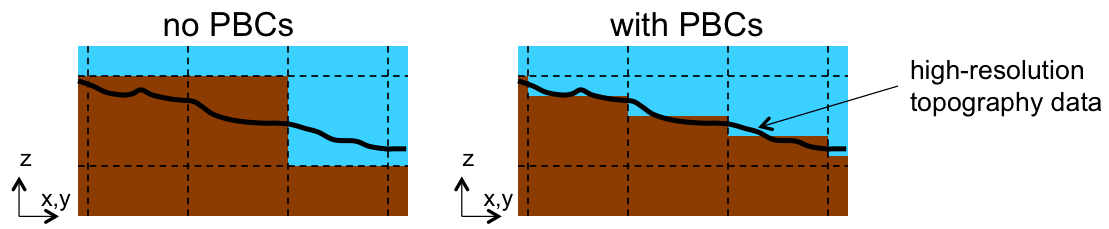
\includegraphics[scale=0.4]{ocean/figures/partial_bottom_cells.png}
\caption{Illustration of partial bottom cells.}
\label{oceanFigure:pbcs}
\end{figure}

For typical global domains, the initial condition file includes the following variables:
\begin{itemize}
\item layerThickness: all full cells
\item tracers: values at middle (in vertical) of full cells
\item bottomDepth: depth of column from bathymetry data
\end{itemize}
Note that there is a mismatch in these data fields, because layerThickness and tracers are initialized for full cells, but bottomDepth is from bathymetry and so may fall anywhere within the bottom cell.  This configuration of initial conditions was chosen so that a single file may be used for any PBC setting upon start-up.  These variables are changed for the PBC configuration when starting from initial conditions, and then the PBC settings remain the same for all subsequent restart simulations.  See flags below for a description of how the variables are altered for PBCs.
